\documentclass[11pt, a4paper]{article}
\title{SPS : CW2 Report}
\author{Matthew Duffin}

\renewcommand\thesection{\arabic{section}}
\renewcommand\thesubsection{(\alph{subsection})}

\usepackage[linesnumbered,boxed]{algorithm2e}
\usepackage[margin=2cm]{geometry}
\usepackage{fancyhdr}
\usepackage{graphicx}
%\usepackage{subfig}
\usepackage{titling}

\usepackage{subcaption}

\setlength{\droptitle}{-60pt}

\pagestyle{fancy}
\fancyhf{}
\rhead{md14816}
\lhead{Matthew Duffin}
\cfoot{Page \thepage}

\begin{document}
\maketitle

\section{Introduction}
This report describes the process of desiging a classifier for a set of characters. By extracting features from the fourier space images of these three types of character (S, T and V) I have been able to build a reasonably accurate classifier. 

\section{Feature Selection}
The first step in the process is to find the features that clearly separate the three types of character. We were asked in this task to extract features from the fourier space. As a starting point I created the fourier space images for each of the characters and then took the average of each class. The results of this are shown below. 

\begin{figure}[ht]
\centering
	\begin{minipage}[b]{0.3\textwidth}
		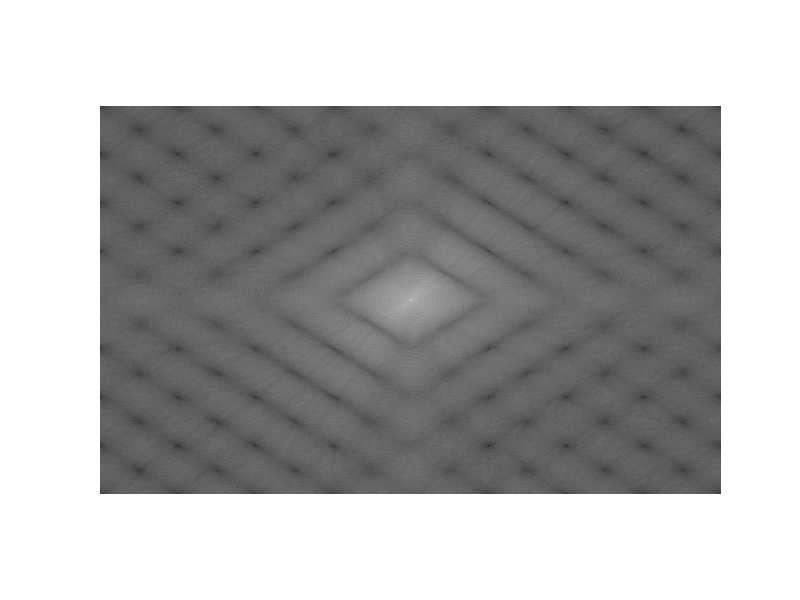
\includegraphics[trim={2cm 2cm 2cm 2cm},clip,width=0.8\textwidth]{characters/S_average.png}
	\end{minipage}	
	\begin{minipage}[b]{0.3\textwidth}
		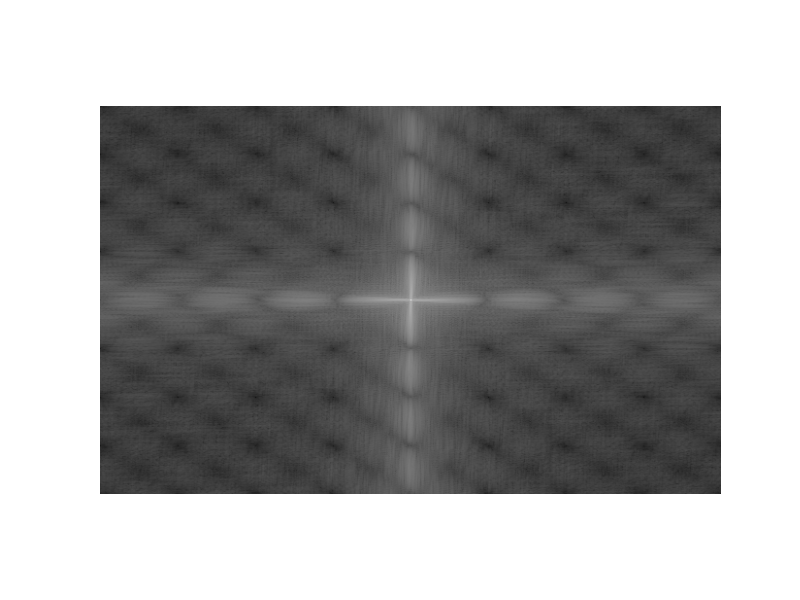
\includegraphics[trim={2cm 2cm 2cm 2cm},clip,width=0.8\textwidth]{characters/T_average.png}
	\end{minipage}
	\begin{minipage}[b]{0.3\textwidth}
		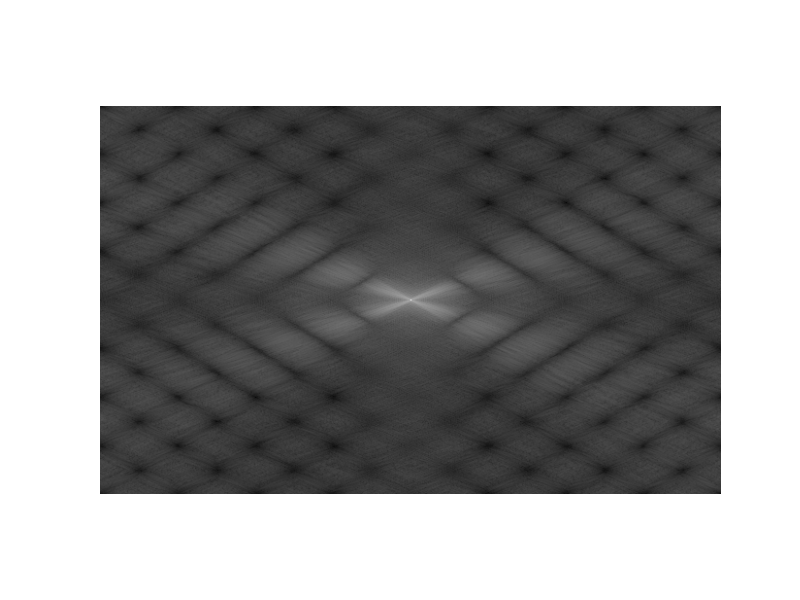
\includegraphics[trim={2cm 2cm 2cm 2cm},clip,width=0.8\textwidth]{characters/V_average.png}
	\end{minipage}
	\caption{Average fourier spaces of S (left) T (centre) and V (right).}
	\label{fig:averages}
\end{figure}

You can see that the fourier space for the letter T has very strong spectral peaks in the horizontal and vertical directions. The vertical line tells us that in the original image there is a high rate of change of intensity in the horizontal direction. The horizontal line shows the same for the vertical direction. Looking at the letter T you can indeed see that the two lines that make it up correspond to the strong bright vertical and horizontal lines in the fourier space. 

At this point I looked at the three images and tried to find regions where the intensity differed. For example, the strong horizontal and vertical lines that are present in the T fourier space are not present in the others. Likewise, the diagonal lines in V's fourier space are not present in the others. Using this information I selected five different regions to take forward and test, which can be seen in Figure ~\ref{fig:features}.

\begin{figure}[ht]
\centering
	\begin{minipage}[b]{0.3\textwidth}
		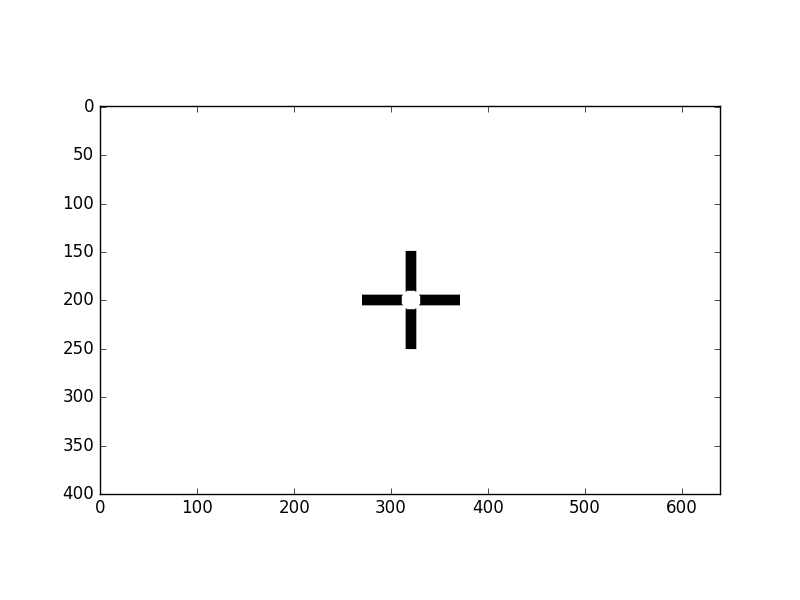
\includegraphics[trim={2cm 2cm 2cm 2cm},clip,width=0.8\textwidth]{features/cross.png}
	\end{minipage}	
	\begin{minipage}[b]{0.3\textwidth}
		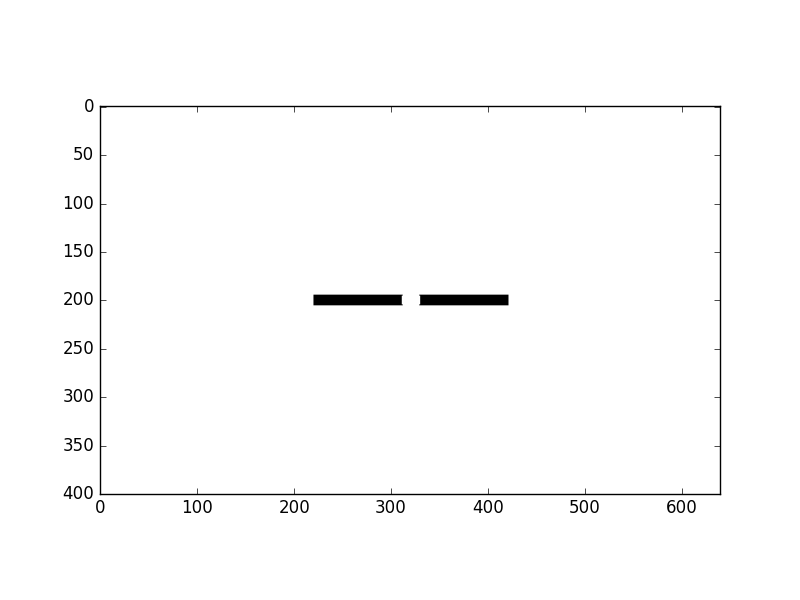
\includegraphics[trim={2cm 2cm 2cm 2cm},clip,width=0.8\textwidth]{features/line.png}
	\end{minipage}
	\begin{minipage}[b]{0.3\textwidth}
		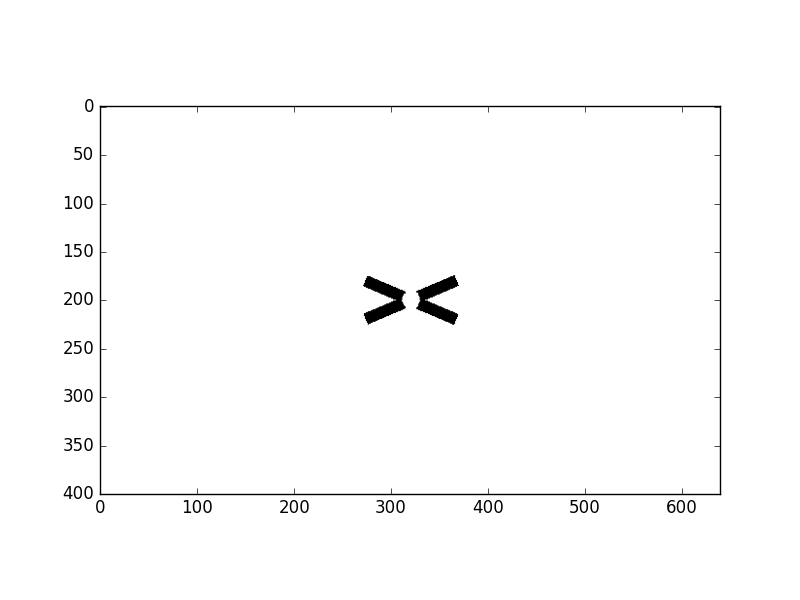
\includegraphics[trim={2cm 2cm 2cm 2cm},clip,width=0.8\textwidth]{features/x.png}
	\end{minipage}
	\begin{minipage}[b]{0.3\textwidth}
		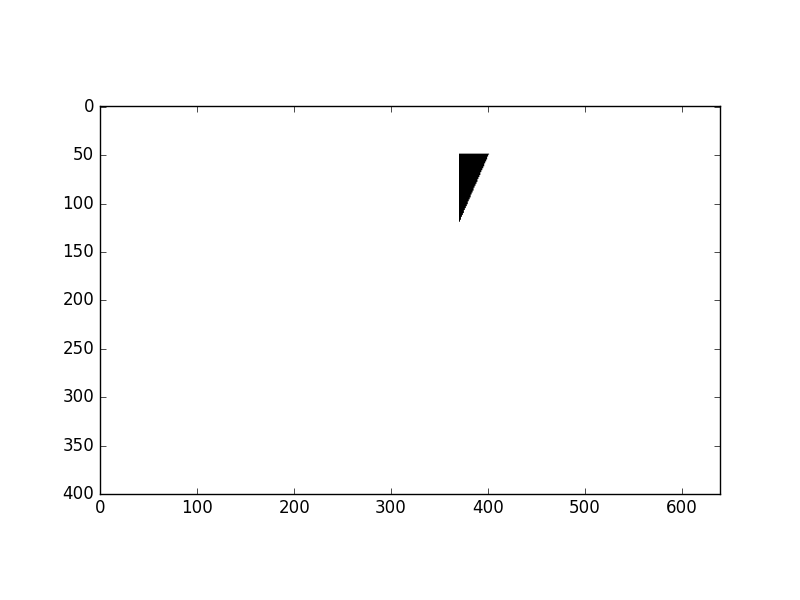
\includegraphics[trim={2cm 2cm 2cm 2cm},clip,width=0.8\textwidth]{features/triangle.png}
	\end{minipage}
	\begin{minipage}[b]{0.3\textwidth}
		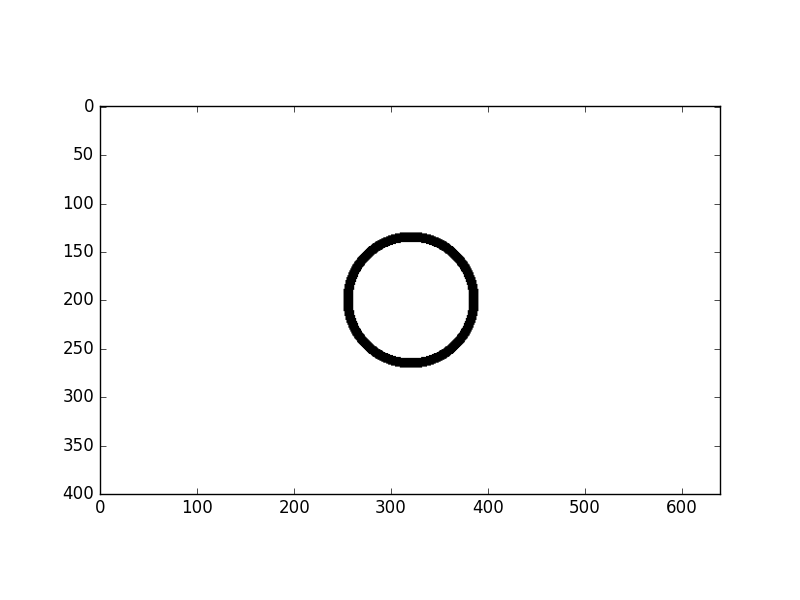
\includegraphics[trim={2cm 2cm 2cm 2cm},clip,width=0.8\textwidth]{features/ring.png}
	\end{minipage}
	\caption{Features selected to take forward to testing.}
	\label{fig:features}
\end{figure}
You will notice that a lot of the features have a "hole" in the middle. This is because I wanted to exclude the DC component from the features. The DC component is the average brightness of the image. It does not give any information about direction. Therefore its inclusion would be likely to skew my results if a certain image were brigher than the others. 

If you look at the 'squashed x' shaped feature you will notice that it very closely follows the shape of the average fourier space for the V images. I measured the angles on frequency domain average to ensure that the correct spectral region was selected.
\begin{figure}[ht]
	\centering
	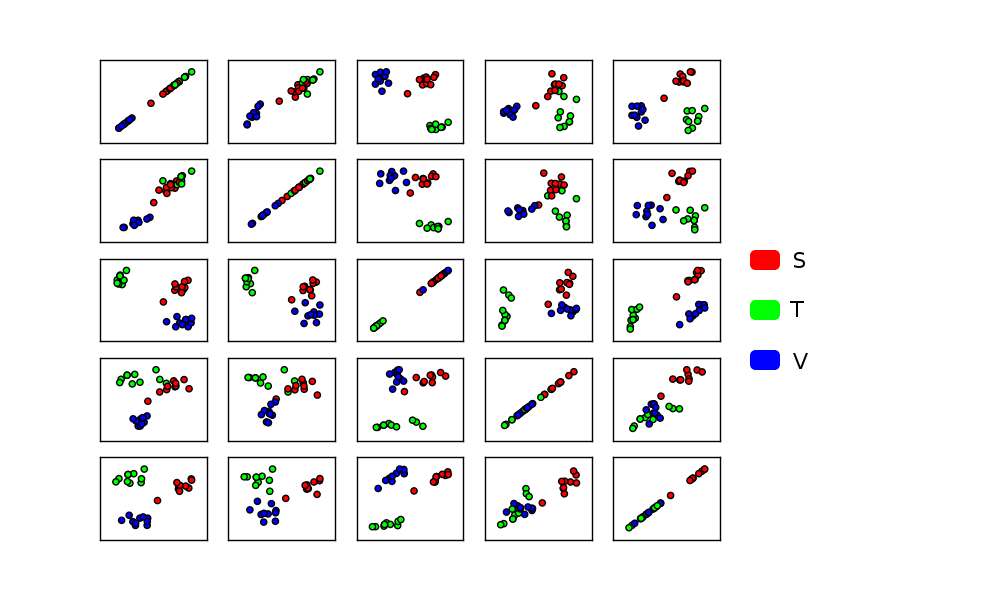
\includegraphics[trim={0 1.5cm 3cm 1.5cm},clip,width=0.75\textwidth]{feature_matrix_leg.png}
	\caption{A grid of plots, each of which plots one feature against another.}
	\label{fig:feature_matrix}
\end{figure}

Next, I took the log of the magnitude spectrum, squared it, and then summed up the region defined by the feature. I took the log in order to reduce the range of magnitudes. Before I took the log I would find certain images had certain regions that dwarfed the rest of the image (around the DC value). By taking the log, the importance of this region was reduced and the importance of the higher frequencies was increased. It is the higher frequencies that are useful in classifying characters. The squaring really doesn't have much of an effect. It spreads out the data slightly more and increases the inter-cluster distance, making the data slightly easier to interpret.

In Figure ~\ref{fig:feature_matrix} I have plotted the features against each other to form a grid of plots. The features are numbered 0 to 4 downwards and 0 to 4 from left to right. There are a number of good candidates, such as (0,2) and (2,4) but I decided to take (0,4) forwards (the cross and the ring) because apart from one wayward point it separates the data into three well defined clusters. A more detailed plot of these two features can be seen in Figure ~\ref{fig:classifier_training}.



% The inter-cluster distance is high so there is a clear separation between clusters. The intra-cluster distances are low though so the underlying gaussian distributions for each cluster have low variance. 

\section{The Classifier}
\subsection{Training The Classifier}

\begin{figure}[!h]
\begin{minipage}[b]{.5\textwidth}
\centering
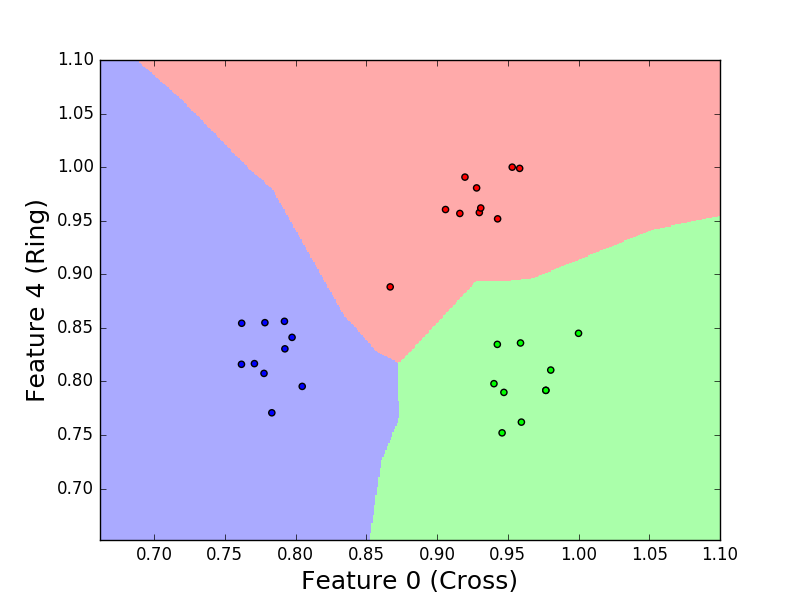
\includegraphics[width=1\textwidth]{training_plot_k1.png}
\subcaption{K=1}\label{fig:traina}
\end{minipage}%
\begin{minipage}[b]{.5\textwidth}
\centering
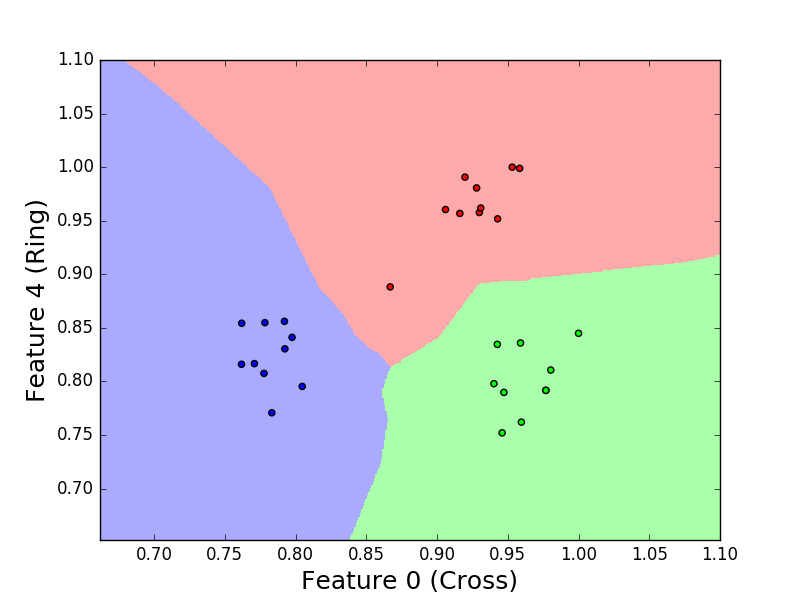
\includegraphics[width=1\textwidth]{training_plot_k2.png}
\subcaption{K=2}\label{fig:trainb}
\end{minipage}
\begin{minipage}[b]{.5\textwidth}
\centering
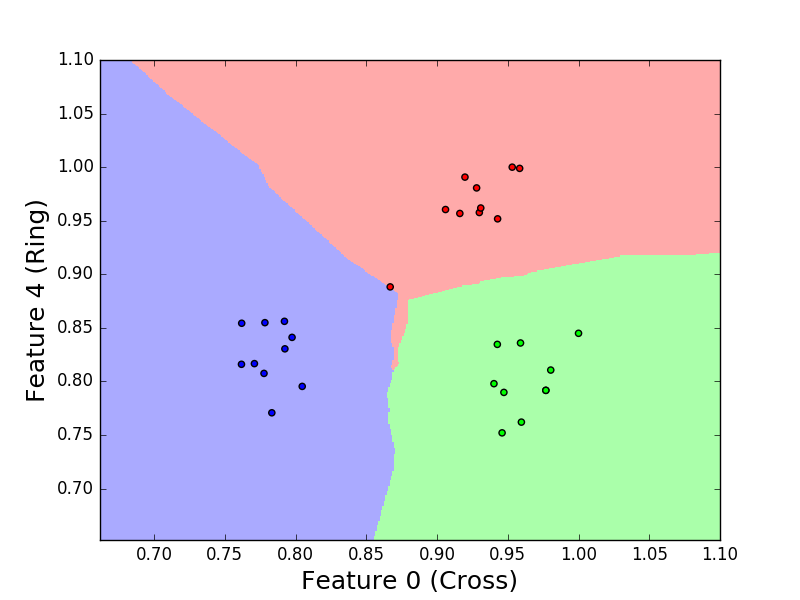
\includegraphics[width=1\textwidth]{training_plot_k3.png}
\subcaption{K=3}\label{fig:trainc}
\end{minipage}%
\begin{minipage}[b]{.5\textwidth}
\centering
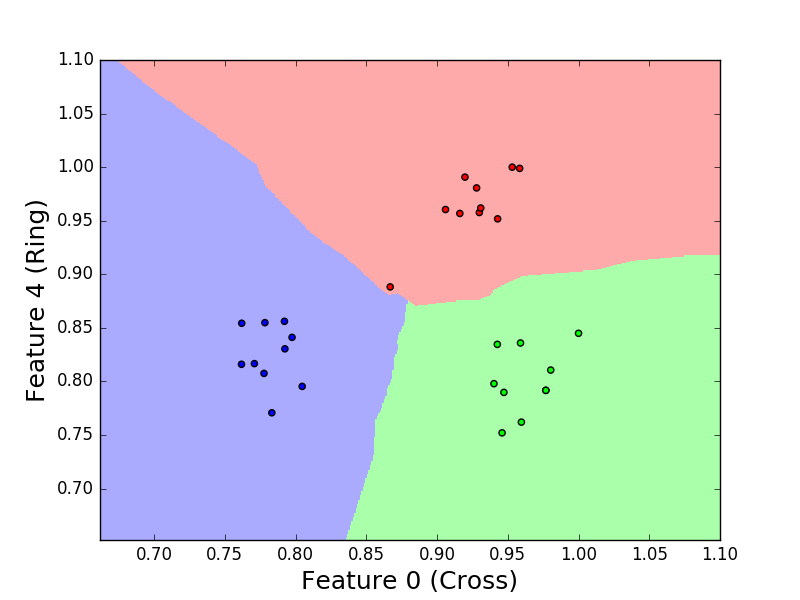
\includegraphics[width=1\textwidth]{training_plot_k4.png}
\subcaption{K=4}\label{fig:traind}
\end{minipage}
\caption{K-Nearest Neighbour Classifiers with K=1..4}\label{fig:train}
\end{figure}

Figure ~\ref{fig:train} shows that the selection of features 0 and 4 was a good one. On these enlarged plots we can clearly see that the inter cluster distance is high, which leads to well-defined decision boundaries. 

I must also mention that the values supplied to the K-Nearest Neighbour  algorithm were normalised first by dividing each feature by the largest value. This had no effect on the classification but just made the scale easier to interpret.

Using K=1 we can see that the one wayward point (one of the S images) massively affects the decision boundary. Opting to use K=1 for our classifier would likely lead to overfitting. 

Looking at the plots showing K>1, you can see that this outlier has less and less of an effect on the decision boundary. At K=4 we see that the decision boundaries are farily straight and look similar to what we would expect from an algorithm such as Nearest-Centroid. 

I chose to use the K=4 classifier due to the reduced influence of the one outlier in the S group. This means there should be a lower chance of overfitting the model to the test data. If a point in my training data were to fall in a similar position, its classification would be viewed with suspicion due to its proximity to the decision boundary. 

\subsection{Testing The Classifier}

In order to test my classifier I produced some images of my own. As well as keeping the same dimensions as the training data images, I tried to match the thickness of the original characters as closely as possible. This is because a different thickness would give a different rate of change of intensity, thus leading to a 'peak' or 'bright spot' in a different region of the frequency domain. 

\begin{figure}[!h]
\centering
	\begin{minipage}[b]{0.3\textwidth}
		
\includegraphics[width=0.3\textwidth]{test/S1.png}
	\end{minipage}	
	\begin{minipage}[b]{0.3\textwidth}
		
\includegraphics[width=0.3\textwidth]{test/S2.png}
	\end{minipage}	
	\begin{minipage}[b]{0.3\textwidth}
		
\includegraphics[width=0.3\textwidth]{test/S3.png}
	\end{minipage}	
	\begin{minipage}[b]{0.3\textwidth}
		
\includegraphics[width=0.3\textwidth]{test/S4.png}
	\end{minipage}
	\begin{minipage}[b]{0.3\textwidth}
		
\includegraphics[width=0.3\textwidth]{test/T1.png}
	\end{minipage}	
	\begin{minipage}[b]{0.3\textwidth}
		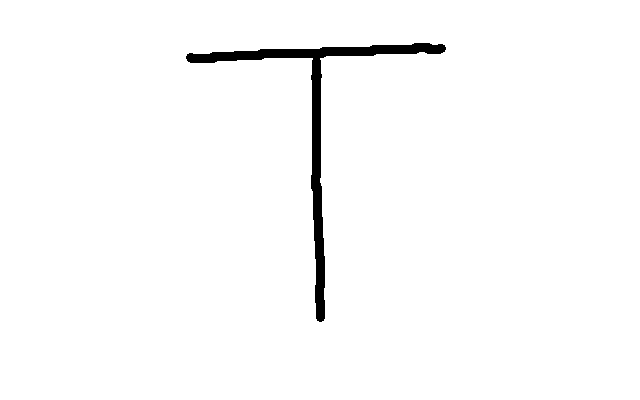
\includegraphics[width=0.3\textwidth]{test/T2.png}
	\end{minipage}	
	\begin{minipage}[b]{0.3\textwidth}
		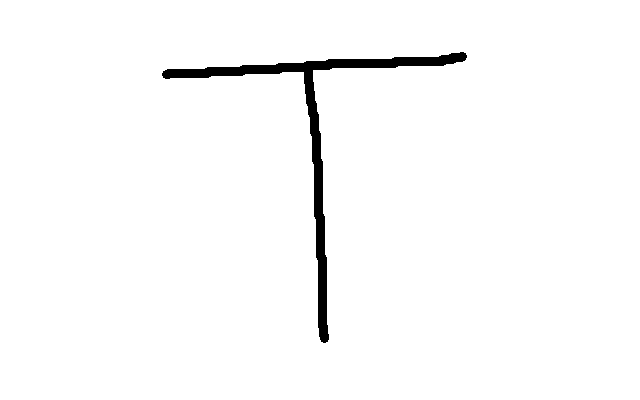
\includegraphics[width=0.3\textwidth]{test/T3.png}
	\end{minipage}	
	\begin{minipage}[b]{0.3\textwidth}
		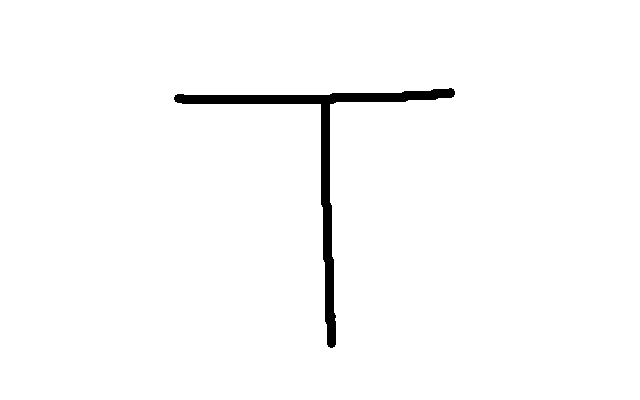
\includegraphics[width=0.3\textwidth]{test/T4.png}
	\end{minipage}
	\begin{minipage}[b]{0.3\textwidth}
		
\includegraphics[width=0.3\textwidth]{test/V1.png}
	\end{minipage}	
	\begin{minipage}[b]{0.3\textwidth}
		
\includegraphics[width=0.3\textwidth]{test/V2.png}
	\end{minipage}	
	\begin{minipage}[b]{0.3\textwidth}
		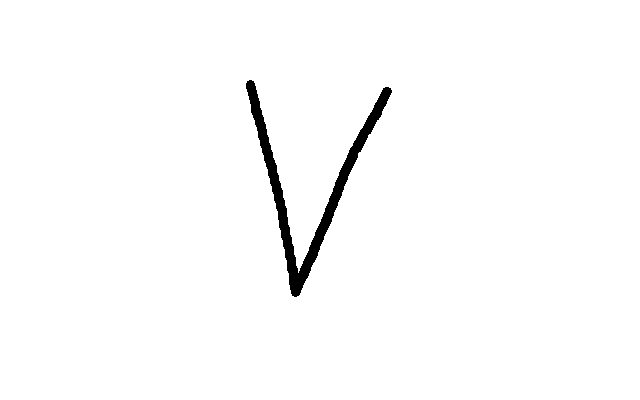
\includegraphics[width=0.3\textwidth]{test/V3.png}
	\end{minipage}	
	\begin{minipage}[b]{0.3\textwidth}
		
\includegraphics[width=0.3\textwidth]{test/V4.png}
	\end{minipage}	
	\caption{Characters produced by myself to test my classifier.}
	\label{fig:test_characters}
\end{figure}

\begin{figure}[ht]
	\centering
	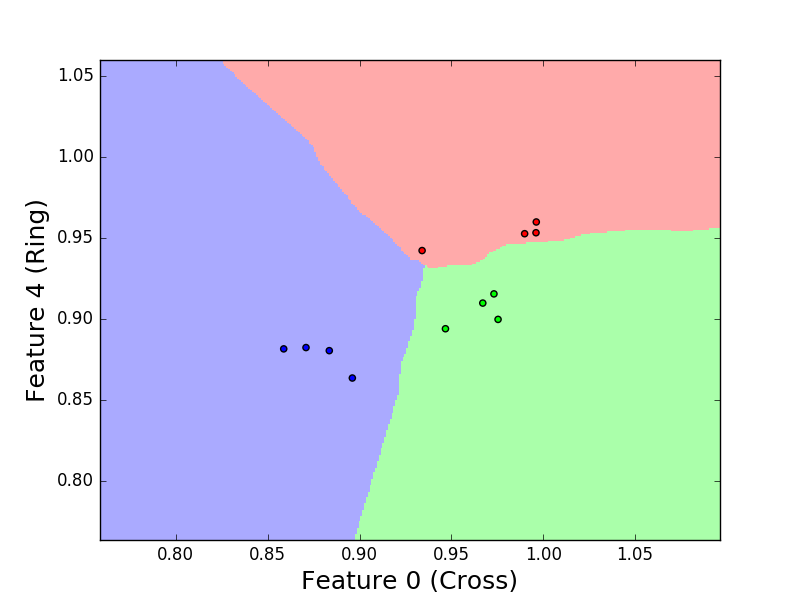
\includegraphics[trim={0 0 0 1cm},clip,width=0.75\textwidth]{test_plot.png}
	\caption{The test data plotted on the The K-Nearest Neighbour classifier with K=4.}
	\label{fig:classifier_test}
\end{figure}

If you look at Figure ~\ref{fig:classifier_test} you can see that all of the test images have been accurately classified. However, the S images have lower feature 4 (ring) values than the training data did. All of the S data points are very close to the decision boundary. This means you would have low confidence in the classification if you did not know which class the data was drawn from, as we do currently in this testing situation. 

Overall I would call this a successful classifier. The only slight issue is the low feature 4 values and high feature 0 values of most of the data points in the S data set. This could be due to the fact that I was using a mouse and trackpad to produce the test images. Writing on paper or a pen tablet, one would be able to produce smoother lines. The 'blocky' nature of my drawing would account for the high feature 0 values, which shows the presence of horizontal and vertical frquencies. 

\section{Classification Of 'A' And 'B' Characters}

In this section I took the classifier that I developed and applied it to two images: an 'A' character and a 'B' character. You can see the results in Figure ~\ref{fig:ab}.

\begin{figure}[h]
	\centering
	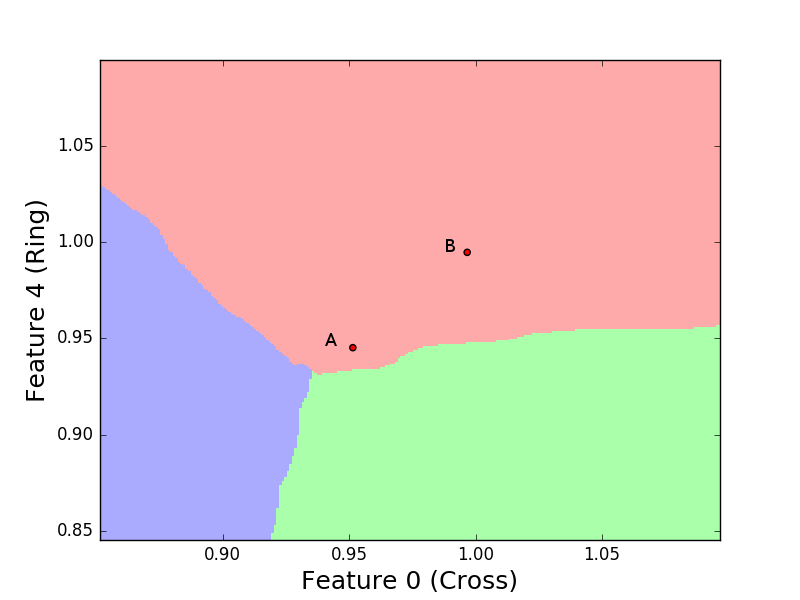
\includegraphics[trim={0 0 0 1cm},clip,width=0.75\textwidth]{ab.png}
	\caption{The classifier applied to images of the characters 'A' and 'B'.}
	\label{fig:ab}
\end{figure}

The results surprised me. The character A was classified as an S, even though it is comprised of two long diagonal lines and a horizontal line. Instead I expected it to be classified as a V. I suspect that the presence of both horizontal and diagonal lines 'filled up' the ring feature enough to push it up above the decision boundary into the S region. 

The letter B was classfied as expected. The curved lines are very similar to the letter S and it was classified as an S accordingly. 

\section{Maximum Likelihood Classifier}
\begin{figure}[ht]
	\centering
	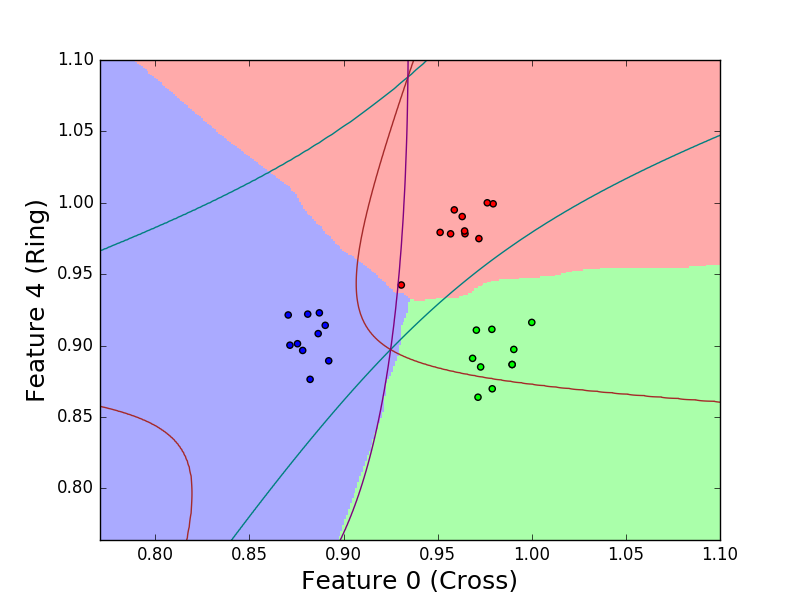
\includegraphics[trim={0 0 0 1cm},clip,width=0.75\textwidth]{max_likelihood.png}
	\caption{A Maximum Likelihood classifier, overlaid on the Nearest Neighbour classifier for comparison. There are three decision boundaries. The teal is betweeen S and T, the purple is between T and V and the brown is between V and S.}
	\label{fig:ml}
\end{figure}

\begin{figure}[ht]
	\centering
	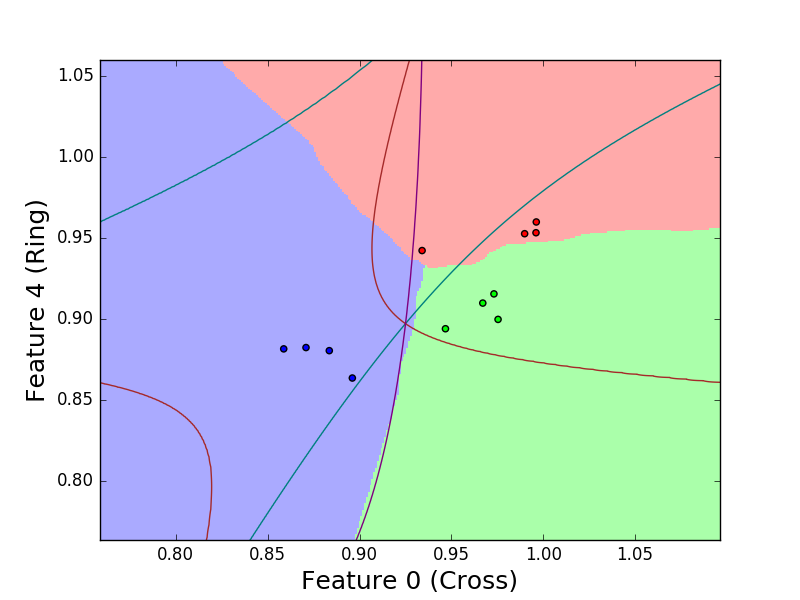
\includegraphics[trim={0 0 0 1cm},clip,width=0.75\textwidth]{max_likelihood_test.png}
	\caption{The same as Figure ~\ref{fig:ml} but showing the test data instead of the training data.}
	\label{fig:ml_test}
\end{figure}

Here I have applied a maximum likelihood classifier to the dataset. I have modelled each group of characters as being generated from a 2D Normal Distribution. The decision boundary is at the locus of points where the probability of belonging to either of the distributions is equal. Either side of the line the probability of belonging to one of the distributions is greater.

I have overlaid these new decision boundaries on top of the Nearest Neighbour decision boundaries. As you can see they differ greatly. The boundary between T and V is fairly similar but the other two are very different. This is due to the influence of the outlying point in the S dataset. This has caused a large variance and has shifted the mean away from the main group. The decision regions are hyperbolic because the covariance matrices of the distributions are not equal. This causes non-contiguous decision regions, as evidenced by the decision boundaries in the bottom left and top left. 

Looking at Figure ~\ref{fig:ml_test} you can see that the classifier has mis-classified three of the four points in the S dataset. This is worse than the Nearest Neighbour classifier. However, the points are still close to the decision boundary, so this would cast doubt on the classification. With more test data we could more accurately compare the two classifiers. 

\end{document}